\section{Satisficing vs Optimizing}
Genetic algorithms are favorable because they provide a good solution to the exploration/exploitation trade-off. If not hunting for a new prime number few are able or willing to wait out their whole lifespan to obtain the scientific results that there career depends on. There are steeply limited budgets for exploring solution spaces, therefore it seems prudent to accept solutions which are are not optimal but are negligently close to optimal. Often however, we may be interested in problems with complex and unlearn-able error surfaces that effectively "bury" the optima in noise. In such a cases it may be acceptable to obtain merely a satisfactory solution, in this context, the highest objective is to recover "biologically plausible models" and many fitted models can easily surpass this lower criteria of acceptable optimization.

Fortunately the coupling of Neuronunit to a Genetic Algorithm facilitates either optimizing or a silent falling back to satisficing as appropriate. The term "satisfice" means that a measured property is either deemed satisfactory or optimal \cite{simon1956rational}. Although we may not know if a true optima is missed, neuronunit is often able to report if a solution is satisfactory. Forinstance when using neuroelectro data we can check if a model is biologically plausible, by consulting the models $\chi^{2}$ statistic over a collection of different electrical measurements.  Assuming that underlying experimental data is normally distributed as discussed in \ref{section:data-sources}. In addition to near optimal and satisfactory model fits models may also fail to achieve even a satisfactory fit and in that case it is helpful to quantify the degree of fitness failure.

\section{Feature Calculation Algorithm That Unifies Diverging Laboratory Practices}
The NeuronUnit core, the Ephysiology Feature Extraction Library \cite{EFEL}) EFEL, the Allen SDK, and the tests derived from \cite{druckmann2008evaluating} all contain independently written algorithms for computing features from simulated membrane potentials.
In some cases, the same feature (e.g. action potential threshold) is computed in many different ways across these feature extraction libraries.
All compute the threshold by first taking the first difference of the membrane potential, but they differ in subsequent steps, for example what value the first difference must reach to be considered at or beyond threshold.
This is inconvenient, but one can simply select one (or more) of the alternatives and apply it consistently.
More troubling are the cases where these algorithms differ in the stimulus used to generate the feature.
For example, the suprathreshold tests of \cite{druckmann2008evaluating} are based on a multiple of rheobase (e.g. $1.5\times$ or $3\times$), whereas those used by The Allen Insitute are based on additive increments from rheobase (e.g. +20 pA or +40 pA).
This means that cannot simply be applied to the same membrane potential trace, as those who collected the experimental data are likely to have chosen either multiples or additive increments of rheobase, but not both, depending on which lab they happen to work for.

As discussed in \ref{sec:methods}, I use code to restructure Allen and BlueBrainProject sweep data sets, where I sort traces into approximate multiples of rheobase. To make these conflicting lab protocols interoperable I impute 1.5 $\times$ and 3 $\times$ rheobase where it was not provided by finding the stimulus sweep pair that is the closest approximation. In this way I find the nearest traces to those predicted values in the Allen and BBP collections of sweeps. However, one can conceive of more mathematically savvy types of imputation, that achieve much greater levels of accuracy by weighting components of the two closest waveforms together, according to eachs distance from the required current injection value. In this way I assumed it was possible to generate predicted features from one stimulus convention based on observed features from the other, meaning that via imputation I had obtained an full (but approximated) set of features across the differing lab protocols.

%that is what I mean when I write imposing a new organisation on the sweep data.

% It may be possible to generate predicted features from one stimulus convention based on observed features from the other, allowing imputation of a full set of features across all algorithms, but this is beyond the scope of my thesis work. ISNT THIS WHAT I DID IN SOMEWAYS? IF I COULDN"T COMPARE ACROSS LAB PROTOCALS THEN THE ANALYSIS I DID WAS POINTLESS WAS IT NOT?

\section{Cross-Validation for Feature Selection.}
The features identified during multivariate analysis utlilized the entire collection of models, data, and stimuli.
By constrast, a machine learning approach would have held out some of these for cross-validation, checking to see whether the features identified on a training set were in fact that features that best cluster, discriminate, or simply explain variance in the a held-out set of models and data.
For example, future work could identify a canonical set of stimuli and features fitness criteria, criteria that can train models to best satisfy multiple experimental protocols, rather than just one particular experiment.

The approach would involve starting with a wide set of above and below threshold experiments, and systematically shuffling the objectives into ``validation" and ``train" sets. The GA only fits to constraints that belong to the training set, after fitting trained models are evaluated against left over validation constraints.

Cross-Validation may provide a strategy for dealing with conflicted fitness criteria, such as the input resistance test. If models fail to recapitulate a test, beyond the insight that fitted reduced models don't agree with input resistance experiments. We want to know if training models to fit tests that they can't align to, harms the models ability to satisfy the other tests. If its the case that trying to satisfy input resistance tests, harms the generalizability of a model, it would might be better to document the model weakness, and drop input resistance from future collections of optimization constraints.

\section{Which is the best model to optimize with?}
Multi-time scale variants of the adaptive exponential model also won, the INCF competition \cite{incf_multi}.

Generally the Izhikevich model was the overall winner, as when averaging across $\chi^{2}$ statistics for 8, tests, the Izhikevich model had the lowest mean $\chi^{2}$, and the highest average $p-value$ however, when regarding each data set as a novel contest, the Adaptive Exponential lost to the Izhikevich model on two or more data sets see appendix \ref{appendix}.
Adexp $28.55$ versus 
Izhikevich $1.39$
The problem was that the Adaptive Exponential failed to find biologically plausible fits on most of the Neuroelectro data sets: olfactory mitral cell and Cerebellum Purkinje cell. however, if you remove these two difficult data sets, and then judge models on 6 of the 8 remaining tests, then the adaptive exponential has the lowest mean $\chi^{2}$ statistic. $AdExp=0.51$	$Izhikevich=0.99$.

Like the AdExp cell, GLIF cell had success only if you consider limited ranges of data. If you consider only Allen cell types sources of data, then the GLIF cell has $\chi^{2}$ values as slightly lower than $1.0$ GLIF 4 Allen Tests only, however, if you include all the 8 tests, then the mean $\chi^{2}$ value is very high. $364.15$

The GLIF cells were able to recapitulate FIslope exactly, however, this caused conflicts with ability to fit time constant, and rheobase values.

The GLIF model was able to optimize cells to be within the biologically plausible range $\chi^{2}<1.0$, however these models were slow, unless $dt>=0.5ms$. and the quality of fits was not astounding, given such slow simulator convergence.

As discussed in methods the Izhikevich model consisted of $4$ different equations, it is of interest to know, if allowing the optimizer access to the broader range of firing regimes improved electrical fits. After consulting the results see \ref{appendix}, we found that in fact, all regime related sub-types were used. Specifically excepting for model $6$ (TC - Cat dorsal LGN thalamocortical cell) all other sub-types of the Izhikevich were sampled and ultimately utilized by the optimizer to achieve best fits. With $4$ Rat barrel cortex Low-threshold  spiking (LTS) interneuron 
$5$ FS - Layer 5 rat visual cortex fast-spiking (FS) interneuron, used the most often. Regimes $1-3$ in this case representing the "regular-spiking" regime. A little surprisingly the regimes $1-3$ were only used in one fit Allen specimen $id-623960880$.

\section{Parameter Boundaries}
When setting parameter boundaries there is a dilemma: If the upper and lower parameter margins are closer together than necessary, then optimized models may be deprived of the range they need to reach their best fit. On the other hand if the boundaries are too far apart, then the governing equations of the model may yield unstable solutions, which may impair the error surface as I will describe below.

Error surface tractability can be compromised in two ways.
Type \textbf{1} solutions to governing equations may contain "not a number" (NaN) or infinity value. The optimizer conventionally interprets more positive numbers as worse. Inside the optimization framework infinity or NaN values are converted to a nominal value of $100.0$, the worst conceivable model score. If more than one gene scores at $100$, then there will be regions of flat error surface. %Although genetic algorithms are not pre-determined to take the steepest path down an error slope, 
%All optimization algorithms are sensitive to the informativeness of error surface, therefore a flat error surface is unhelpful in both gradient descent and genetic algorithms, 

\begin{figure}
    \centering
    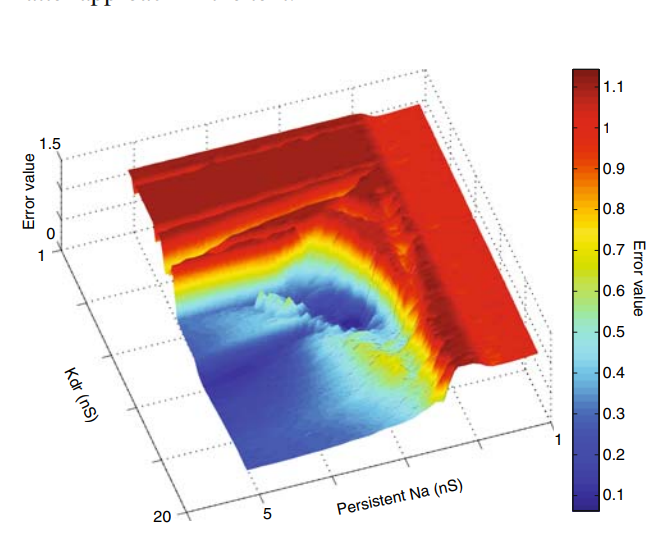
\includegraphics[scale=0.65]{figures/cliff.png}
    \caption[A plot of a cliff ledge framing a 2D error surface]{A plot sourced from literature:
\citep{van2007neurofitter,van2008automated}. This is a plot of summed error across a 2D surface, where swept values of $N_{a}$ conductance form the x-axis, and $K_{dr}$ conductance form the y-axis. Between Na $[1-5]$, you can observe that Na retains a flat value. Presumably the high flat error acts to frame the viable middle region of model parameters, by excluding unstable models.}
    \label{fig:best_at_edge}
\end{figure}
When error surface is flat it is uninformative. Flatness in the viable middle region of optimization, is usually unhelpful, but there is one important place where flatness is helpful. It is warranted for the middle region of error space to be framed by cliffs that demarcate a non-viable perimeter of the error hyper-volume, these are the regions where model parameters are operating slightly beyond their intended scope. There is evidence this approach is used in other optimization work.


\begin{figure}
    \centering
    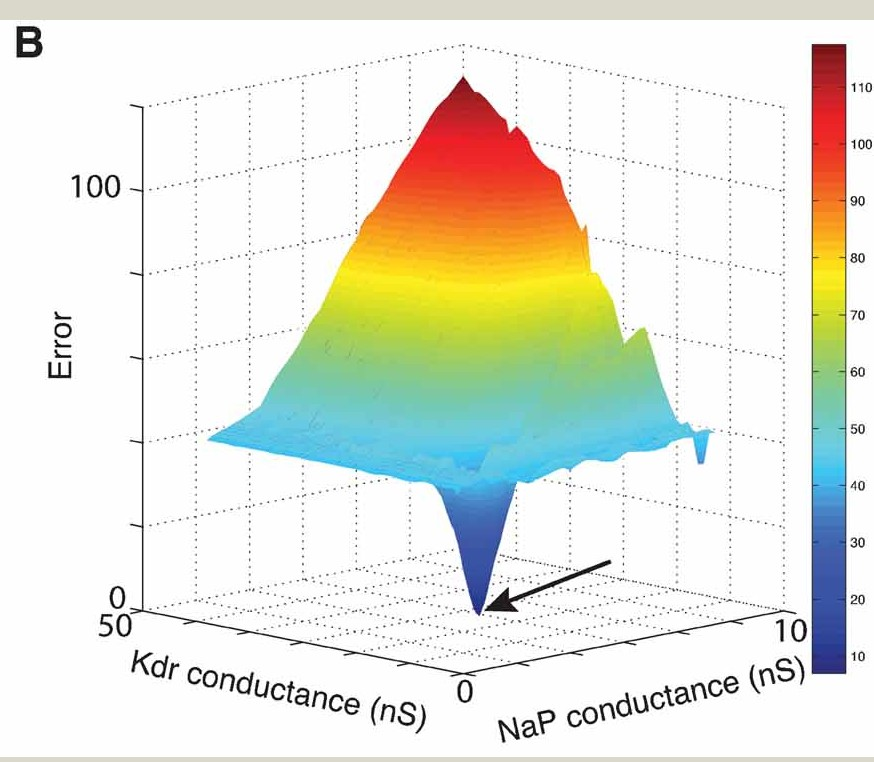
\includegraphics[scale=0.65]{figures/fninf-01-001-g009.jpg}
    \caption[An optimal value that would be missed using only a slim parameter range]{
    Again from the literature I provide a plot of error surface for reduced neuronal models
    \citep{van2008automated}
    \citep{van2007neurofitter}}
    \label{fig:best_at_edge}
\end{figure}

Consider \ref{fig:best_at_edge}, in this figure a global minima is positioned at the intersection two parameter edges in both $Kdr$ and $NaP$. It would be easy to formulate the same optimization problem to have truncated scope about the extremes of $NaP$ and $Kdr$ and as a consequence to miss the uniquely positioned global optima situated on the intersection. The alternative optima that would be reported is the broad spanning region that shares the same second lowest value to the optima. 

%The genetic algorithm
As discussed, model-solution instability can occur when the optimizer samples model parameters that are outside of the models intended scope, or when a model returns a nan value inside its intended scope. It is tempting to think of 

Usually these flat cliffs that neatly encase the error hyper volume like in the figure below \ref{fig:cliff} (and as described above).

% Not helpful for audiance to understand.
%unfortunately however, because each model has a large number of parameters typically $>10$, any particular model instance, only one of these parameters need be evaluating an unstable model when exceeding a margin, the rest of the parameters may be in the middle of their range, and so such a ledge may mostly be experienced as a hyper dimensional "tower", this tower could actually be experienced in the middle of parameter space in 10 out of 11 parameters, while still being on at the edge for only the 11th parameter. The unfortunate consequence of such towers is to lesion in the middle of parameter space inhibits the migration of chromosomes between regions. 

From one perspective, the genetic algorithm is robust, and any middle region discontinuities are usually only a temporary hindrance that slows down learning without stopping it completely. From another perspective there are is only a small number of samples that occur inside the GA framework, and it would be better if the occurrence of lesions in the middle of the error surface were reduced to maximize the informativeness of every precious sample. 

The major strategy for circumvent unnecessary ridges and towers is to pick and chose error functions sparingly and to assess results in a piecemeal basis. Utilizing a "sparing" inclusion policy will have to occur despite the large conflicting incentive to employ as many objective functions as possible.

% Picking the right objective functions will likely involve favoring a-posteri evidence over a-priori arguments about which errors "should" work best. 

%the majority of samples in the middle of the error space.

To supplement figures from the literature, here I include some figures from problems encountered in this work.

Although we are considering single points, and not surfaces, very often if a point is unstable, its neighbours are also unstable, in this way points of instability tend to be a constituents of larger regions of surface that add up to towers, cliffs and ledges such as those in seen here {fig:cliff}.

One or more cliffs or towers situated in the middle of the error surface, poses problems for efficient optimization, where genes learn the general shape of an error surface. %Such cliffs and ledges will mislead the optimizer and they will act exactly like the ripples discussed briefly before in this work.

%Type \textbf{2}: While some towers can be circumvented by choosing slimmer parameter margins, other ledges and ripples of these ledges are implied by the types of model and test combinations. Rather than being avoidable, they are a feature of the complex problem that the optimizer is tasked with solving.

Forinstance, in bursting regimes of the Izhikevich model, where models deliberately produce close to unstable limit cycles. When surpassing the threshold to cause spiking, the slightest increment of current  will illicit not a single spike but a burst of ten.

Rheobase values will be undetermined, because the a  current injection value to that causes only one spike does not exist. The models rheobase value will be assigned to 100, and a tower will punctuate, the error surface possibly in the middle of the Izhikevich parameter hypervolume. The experience of sampling this tower, will visible in evaluation of the  algorithms learning performance. It will likely appear as a one or several unexpected peaks late in the genetic algorithms learning. Also this tower may act to lesion error surface, and to inhibit the movement of chromosomes across the solution space.

This means that even under the most tractible conditions when evaluating the performance of genetic algorithm learning, the rapidity of genetic convergence will vary depending on which constraints are chosen, and the regime that the neuronal model is currently sampling from (the models parameters). There will be regions of genetic learning when models will encode high local pockets of error, or "towers" in the middle of the hyper-volume, and if these towers are significantly wide or densely populated, the genetic algorithms learning will be visibly diminished to a random sampling algorithm. What is more, these discontinuties under some circumstances may act to lesion error surfaces and inhibit migration of models from side to side. Movement over cliffs of course will still ultimately occur due to stochastic pressure in gene mutation.

A possible solution to the dilemma of narrow parameter boundaries is to write an algorithm that slowly samples models by expanding beyond overly limited parameter boundaries, and reports back on model stability. In this manner one can do obtain the maximum parameter boundaries in an supervised computer algorithm, however, model equations used here, do exhibit some higher order sensitivity by changing a second intermediate parameter. Very quickly this approach to finding the maximum scope of a parameter may begin to look like exhaustive search.

Another programmatic approach is to use a wide variety of models and tests, and to accept that for some model-test combinations, for some regions of parameter space, genetic algorithms are at worst randomly stumbling upon satisfactory solutions, and at best efficiently learning the optima solutions.
